\section{The Higgs Mechanism with Lagrangians*}
\subsection{Intro}
This is a re-telling of the same story as in the previous section, but by other means. You might find it useful, especially if you are familiar with the concept of Lagrangians. But this is beyond the scope of the course. 
\subsection{Lagrangians}
The Standard Model is a quantum field theory of particles, which is described by a Lagrangian. We did not need that Lagrangian so far, neither did we need to think of particles as fields, but for describing the Higgs mechanism, this kind of language is very useful.

A field in its ground state is usually 'switched off', i.e. its value is $0$. Particles are excitations of this field.

The nice thing is that, once you understand Feynman diagrams, you can easily "read" a Lagrangian. The rules are:
\begin{itemize}
\item The Lagrangian for a free (no interactions) fermion of mass $m$ is: 
\begin{equation}
\bar{\psi} i\left(\gamma^0\frac{\partial\psi}{\partial t}-\vec{\gamma}\cdot \vec{\nabla}\right)\psi
 - m \bar{\psi} \psi
\end{equation}
where $\overline\psi \equiv \psi^{\dagger} \gamma^0$ (this is chosen because $\overline{\psi}\psi$ is a Lorentz-invariant quantity, while $\psi^{\dagger}\psi$ is not) which looks, of course, very similar to the Dirac equation. Note the mass term $ - m \bar{\psi} \psi$. This tells you what the propagator of this field is!
\item The Lagrangian for neutral boson, which can be described by a real...
\begin{equation}
\half \left|\frac{\partial}{\partial t} \phi \right|^2
-
\half \left|\vec{\nabla}\phi\right|^2
 - \half m^2|\phi|^2
\end{equation}
... or a complex field:
\begin{equation}
\label{eq:LagrangeComplex}
\left(\frac{\partial}{\partial t} \phi^{*} \right)
\left(\frac{\partial}{\partial t} \phi \right)
-
\left(\vec{\nabla}\phi^{*}\right) \cdot \left(\vec{\nabla}\phi\right)
 -m^2\phi^{*}\phi
\end{equation}
Note the mass term $ - m^2 \phi^*\phi$. We generalise from these examples that mass terms always have two fields!
\item Interactions between fields come from terms with 3 or more fields. This term $g \phi \theta \psi$ for example corresponds to a vertex in a Feynman diagram like this\\
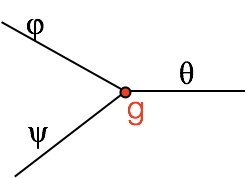
\includegraphics[width=0.2\textwidth]{fig/Feynman3}
\end{itemize}
So for example, this:
\begin{equation}
\mathcal{L} = 
\bar{\psi} i\left(\gamma^0\frac{\partial}{\partial t}-\vec{\gamma}\cdot \vec{\nabla}\right)\psi  - m \bar{\psi} \psi
%
+
\half \left|\frac{\partial}{\partial t} \phi \right|^2
-
\half \left|\vec{\nabla}\phi\right|^2
 - \half \mu^2|\phi|^2
%
+ 
g \bar{\psi}\psi\phi
%
\end{equation}
describes a world with two types of particles, a fermion with mass $m$ and a neutral boson with mass $\mu$. There is one interaction vertex that looks like this:
\\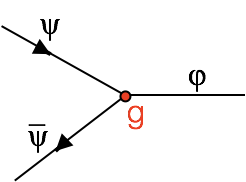
\includegraphics[width=0.2\textwidth]{fig/psibarpsiVertex}\\

\subsection{Gauge invariance}
Gauge invariance is an important principle in particle physics. We all know that in quantum mechanics, phases don't matter. And indeed, our Lagrangians above are all invariant under transformations like $\psi \to \psi e^{i\chi}$, where $\chi$ is a phase, that does not depend on position or time (i.e. a "global" phase).

We now demand that the Lagrangian remain invariant under \emph{local} phase transformations $\psi \to \psi^{iq \theta(x)}$ where, importantly, $\frac{\partial}{\partial t} \theta \neq 0, \vec{\nabla} \theta \neq 0$ (and $q$ is a constant factor we put in for future convenience). Why this is a good thing to demand is not at all obvious. But it turns out that doing so seems to lead to theories that describe nature. One advantage of gauge theories is that they are normalisable, which means we know how to calculate higher order diagrams (this insight won t'Hooft a Nobel Prize). So let's just go with it. Terms like these:
\(
\overline{\psi} \psi
\)
are gauge invariant because
\begin{equation}
\overline{\psi} \psi \to
\overline{\psi e^{iq\theta(x)}} \psi e^{iq\theta(x)}
=\overline{\psi} e^{-iq \theta(x)} \psi e^{iq\theta(x)}
=\overline{\psi} \psi
\end{equation}
while terms with derivatives like
\(
\bar{\psi} i\left(\gamma^0\frac{\partial}{\partial t}-\vec{\gamma}\cdot \vec{\nabla}\right)\psi
\)
are not, because
\begin{align}
\overline{\psi e^{iq\theta(x)}} \left(i\gamma^0\frac{\partial}{\partial t}-\vec{\gamma}\cdot \vec{\nabla}\right)\psi e^{iq\theta(x)}
& =
\bar{\psi} i\left(\gamma^0\frac{\partial}{\partial t}-\vec{\gamma}\cdot \vec{\nabla}\right)\psi
- \bar{\psi} \left(\frac{\partial q\theta(x)}{\partial t} - \vec{\nabla}q \theta(x)\right)\psi
\\
&\neq 
\bar{\psi} i\left(\gamma^0\frac{\partial}{\partial t}-\vec{\gamma}\cdot \vec{\nabla}\right)\psi .
\end{align}
Gauge invariance can be recovered by substituting 
\begin{align}
\label{eq:recoverGaugeInvariance}
    \frac{\partial}{\partial t} &\to 
    \frac{\partial}{\partial t} + i q V
    &
    \vec{\nabla} &\to
    \vec{\nabla} + iq \vec{A}
\end{align}
where $V$ and $\vec{A}$ transform like
\begin{align}
    V & \to V -  \frac{\partial \theta}{\partial t}
    &
    \vec{A} & \to \vec{A} - \vec{\nabla}{\theta}
\end{align}
These are the same rules as for gauge transformations of electric and magnetic potentials. In fact $V$ and $\vec{A}$ \emph{are} the electric and magnetic potential. We combine $V$ and $\vec{A}$ to a 4-vector $\mathcal{A}$ which represents the photon. This is how gauge bosons are born: fields introduced to restore local gauge invariance. This example was for a $U(1)$ gauge transformation ($U(1)$ is the group of complex numbers of modulus $1$, i.e. numbers like $e^{i\theta}$), and the resulting gauge theory is quantum electrodynamics (I also set the charge for the fermion field to $1$, in general you'll have some factors of $q$ in these equations). Weak interactions result from demanding gauge invariance under local $SU(2)$ transformations, strong interactions from local $S(3)$ transformations. From the transformation rules above, it is clear that terms like $m|\mathcal{A}|^2$ are not gauge invariant.
\\\fbox{\parbox{0.98\textwidth}{
    No mass terms are allowed for gauge bosons, i.e. photons, $W$, $Z$, gluons.
}}\\
This is of course a big problem, because $W, Z$ do have masses. How do they get them?

\subsection{Rules for terms in a Lagrangian}
Demanding gauge invariance results in the following rules for our Lagrangian:
\begin{itemize}
\item All terms must be charge-neutral and singlets under weak isospin $T$ (i.e. have $T=0$). Remember that weak isospin just behaves like spin, so two spin \half\ fields can combine to spin $0$ and spin $1$ (symbolically: $\half \otimes \half = 0 \oplus 1$). A combination of two such fields would be allowed, because it includes $T=0$. 
Terms with three such fields are forbidden, because $\half \otimes \half \otimes = \half \oplus \frac{3}{2}$. A combination of two $T=\half$ and one $T=1$ field on the other hand is allowed.
\item mass terms for gauge bosons (photon, $W$, $Z$, gluon) are not allowed.
\end{itemize}
What about mass terms for fermions? They look like $-m \overline{\psi}\psi$. Looks OK at first sight - but we there is a problem. Let us write $\psi$ as a sum of its chirality left and right-handed components: $\psi = \psi_L + \psi_R$. $\psi_{L,R}$ can be written as $P_{L,R}\psi$, with the projection operators $P_{L,R} = \half(1 \mp \gamma_5)$ where $\gamma_5 = i\gamma^0\gamma^1\gamma^2\gamma^3\gamma^4$). What we need to know for what follows is: $P_L P_R=P_RP_L = 0$, $P_L^2 = P_L$, $P_R^2=P_R$ (all of this you'd expect from a pair of orthogonal projection operators), and that $\overline{P_{L,R}\phi} = \overline{\phi} P_{R,L}$
Then
\begin{equation}
m \overline{\psi}\psi = m\left(
\overline{\psi}_L\psi_L + \overline{\psi}_L\psi_R + \overline{\psi}_R\psi_L + \overline{\psi}_R\psi_R\right)
=
m \overline{\psi}_L\psi_R + m\overline{\psi}_R\psi_L
\end{equation}
%
This means that mass terms for fermions \emph{always} involve a mix of left- and right-handed fields.
%
Why is this a problem? It is because in the SM, they have different weak isospin: $\psi_L$ has $T=\half$ while $\psi_R$ has $T=0$. So a term like $m \overline{\psi}_L\psi_R$ cannot be $T=0$.
So these terms are not allowed. This means:
\\\fbox{\parbox{0.9\textwidth}{In the SM w/o the Higgs field and symmetry breaking, all particles would be massless}}\\

\subsection{The Higgs field}

Let us add a new field, $\Phi_H$, with $T=\half$. Using Equations~\ref{eq:LagrangeComplex}, and \ref{eq:recoverGaugeInvariance} we can write a gauge invariant term
\begin{equation}
\left(\left(\vII{ \frac{\partial}{\partial t} }{\vec{\nabla}}
- iq\mathcal{A}\right) \Phi_H \right)^{\dagger}
\left(\left(\vII{ \frac{\partial}{\partial t} }{\vec{\nabla}}
- iq\mathcal{A}\right) \Phi_H \right)
\end{equation}
which includes a term
\begin{align}
q^2 \Phi \mathcal{A}^{\dagger} \mathcal{A}
\end{align}

We can also have a gauge invariant term
\begin{align}
\lambda_{\phi} \Phi (\overline{\psi}_L\psi_R + \overline{\psi}_R\psi_L))
\end{align}
where $\lambda_{\phi}$ represents the interaction strength.
%%
So far these two terms represent two vertices, one for $\Psi$ to two photons, one for $\Psi$ to two fermions.
 Usually, a field is zero and its excitations are particles. But what if the field in the groundstate is not zero, $\Phi = \Phi_0 + h$? Now $h$ is the excitation of this field, i.e. a physical particle. And $\Phi_0$ is a constant, called the vacuum expectation value (vev). Our gauge invariant vertex factors now become:
\begin{align}
q^2 \Phi \mathcal{A}^{\dagger} \mathcal{A} &= 
q^2 \Phi_0 \mathcal{A}^{\dagger} \mathcal{A} + q^2 h \mathcal{A}^{\dagger} \mathcal{A} 
\\
\lambda_{\phi} \Phi (\overline{\psi}_L\psi_R + \overline{\psi}_R\psi_L)) &=
\lambda_{\phi} \Phi_0 (\overline{\psi}_L\psi_R + \overline{\psi}_R\psi_L)) +
\lambda_{\phi} h (\overline{\psi}_L\psi_R + \overline{\psi}_R\psi_L)) &=
\end{align}
%
We now have a term that looks exactly like a mass term for the photon \(q^2 \Phi_0 \mathcal{A}^{\dagger} \mathcal{A}\), and one that looks exactly like a mass term for a fermion \(\lambda_{\phi} \Phi_0 (\overline{\psi}_L\psi_R + \overline{\psi}_R\psi_L)\)
%
%
We also have two interaction vertices, \(q^2 h \mathcal{A}^{\dagger} \mathcal{A}\), and \(\lambda_{\phi} h (\overline{\psi}_L\psi_R + \overline{\psi}_R\psi_L)\)
%%
Importantly, for masses generated with the Higgs mechanism, it follows directly from the above that\\
\fbox{\parbox{0.9\textwidth}{
For any particle, the interaction strength with the Higgs boson $h$ is exactly proportional to the mass of the particles}}\\

Now we just created a heavy photon, although of course the real photon is massless. But the same mechanism can be to generate masses for $W$ and $Z$. In case you feel you are getting short-changed: Higgs got his Nobel Prize exactly for showing how to generate heavy photons! The generalisation to $W$, $Z$ came later.

\subsection{Breaking the symmetry}
\begin{figure}
\centering
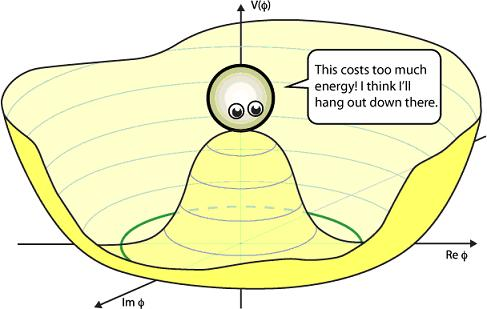
\includegraphics[width=0.45\textwidth]{fig/higgs/phi_unstable.JPG}
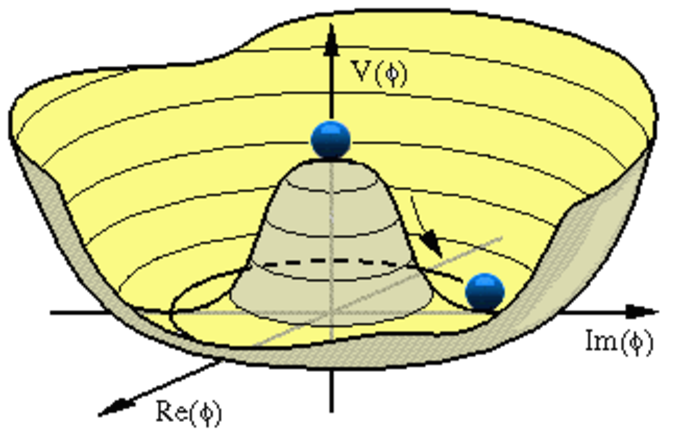
\includegraphics[width=0.45\textwidth]{fig/HiggsAtBottom}
\caption{Higgs potential, with Higgs field wondering where to go, and finally settleing for a ground state.\label{fig:higgPotential}}
\end{figure}
But how do we get the Higgs field to be switched on all the time? We simply postulate that the potential energy of the (complex) Higgs field looks like in \figref{fig:higgPotential}. Notice a crucial feature in that figure: Gauge transformations (in $U(1)$) correspond to rotations in the $Re(\Phi)-Im(\Phi)$ plane. So the potential is gauge symmetric. But the ground state is not. The the original gauge symmetry is still there, but it has been "spontaneously broken" from the perspective of the ground state, the symmetry is not apparent. This resulted in the appearance of massive fermions and gauge bosons.


